\documentclass[UTF8,titlepage]{ctexart}
%\CTEXsetup[format={\Large\bfseries}]{section}
\usepackage{amsmath}
\usepackage{caption}
\usepackage{graphicx}
\pagestyle{plain}
\title{翻译《The Mathematical Theory of Finite Element Methods 3rd Ed (Brenner2007)》 11.3节}
\date{\today}
\begin{document}
\maketitle

\section{有限元近似和锁定}
为简单起见,我们假设$\Omega$是一个凸多边形区域,并且$\Gamma_1$ or $\Gamma_2$中任意一个为空。对于纯位移问题($\Gamma_2=\emptyset$),我们只需考虑齐次边界条件。
\par
令$\emph{T}^h$ 是$\Omega$ 三角划分的一个非退化族。对于纯位移问题($\Gamma_2=\emptyset$),我们使用有限元空间
% \begin{equation}\label{equ1} (\ref{newton})引用
%	V_h := \{ \nu \in H^1(\Omega) : \nu |_{\emph{T}} \mbox{为线性函数}, \forall \emph{T} \in \emph{T}^h \}
% \end{equation}
\\ \\
(11.3.1)
$
	\quad \quad \quad
	V_h := \{ \nu \in H^1(\Omega) : \nu |_{\emph{T}} \mbox{为线性函数}, \forall \emph{T} \in \emph{T}^h \},
$ 
\\ \\
并且对于纯牵引力问题($\Gamma_1 = \emptyset$),我们使用
% \begin{equation}\label{equ2}
%	V_h :=
%\end{equation}
\\ \\
(11.3.2)
$
	\quad \quad \quad
	V_h := \{ \nu \in H^1(\Omega) : \nu |_{\emph{T}} \mbox{为线性函数}, \forall \emph{T} \in \emph{T}^h \},
$
\\ \\
根据第二章和第四章的理论我们得到以下定理。
\\ \\
\textbf{(11.3.3) Theorem.} 令 $u \in H^2(\Omega) \cap H^1(\Omega)$ 满足纯位移问题,并且$u_h \in V_h$ 满足
$$
	a(u_h, \nu) = \int_{\Omega} f \cdot \nu dx \quad \forall \nu \in V_h.
$$
\\
则存在一个正常数$C_{(\mu, \lambda)}$ 使得
\\ \\
(11.3.4)
$
	\quad \quad \quad
	\| u - u_h \|_{H^1(\Omega)} \le C_{(\mu, \lambda)} h \| u \|_{H^2(\Omega)}.
$
\\ \\
\textbf{(11.3.5) Theorem.} 令 $u \in H^2(\Omega)$ 满足纯牵引力问题。令 $u_h \in V_h$ 满足
$$
	a(u_h,\nu) = \int_{\Omega} f \cdot \nu dx + \int_{\Gamma} t \cdot \nu ds \quad \forall \nu \in V_h.
$$ 
\\
则存在一个正常数$C_{(\mu, \lambda)}$ 使得
$$
	\| u - u_h \|_{H^1(\Omega)} \le C_{(\mu, \lambda)} h \| u \|_{H^2(\Omega)}.
$$
对于一般情况 $ \emptyset \ne \Gamma_1 \ne \partial \Omega $ 下的收敛定理,查看练习 11.x.25. 
\\
对于固定的 $\mu$ 和 $\lambda$,定理 11.3.3 和 11.3.5 给出了弹性问题令人满意近似的有限元近似。但是这些有限元方法的性能随着 $\lambda$ 趋向于 $\infty$ 而变差。这就是所谓的锁定现象,我们将在本节的其余部分解释。
\par 
令 $\Omega = (0,1) \times (0,1)$. 我们考虑 $\mu = 1$ 时的纯位移边值问题:
\\ \\
(11.3.6)
$
\quad \quad \quad
\begin{matrix}
	div \{ 2 \epsilon (u^{\lambda}) + \lambda tr (\epsilon (u^{\lambda})) \delta \} = f \quad in \quad \Omega \\ \quad \quad \quad \quad \quad 
	u^{\lambda}|_{\partial \Omega} =  0.
\end{matrix}
$
\\
注意给定的 f ,当 $\lambda \to \infty$,(11.2.33)说明 $\| div u^{\lambda} \|_{H^1(\Omega)} \to 0$.换句话说,我们正在处理一种几乎不可能压缩的弹性材料。为了强调对 $\lambda$ 的依赖,我们将应力张量(11.1.3) $\sigma_{\lambda}(\nu)$ 和 变分形式(11.2.2) $a_{\lambda}(\nu,\omega)$ 表示为
$$
\begin{matrix}
	\sigma_{\lambda}(\nu) = 2 \epsilon(\nu) + \lambda tr (\epsilon(\nu)) \delta \\
	a_{\lambda}(\nu,\omega) = \int_{\Omega} \{ 2 \epsilon(\nu) : \epsilon(\omega) + \lambda div \nu div \omega \} dx.
\end{matrix}
$$

令 $\emph{T}^h$ 为 $\Omega $ (cf.图 1) 的一个规则三角剖分,并且 $V_h$ 被定义为 (11.3.1)。对于每一个 $u \in H^2(\Omega) \cap H_0^1(\Omega)$,我们定义 $u_h^{\lambda} \in V_h$ 为以下方程组的特解
$$
	a_{\lambda}(u_h^{\lambda},\nu) = \int_{\Omega} 
	[ -div \sigma_{\lambda}(u) ] \cdot \nu dx \quad \forall \nu \in V_h.
$$

\begin{figure}[hb]
	\centering
	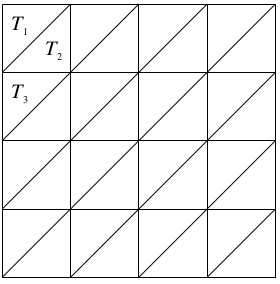
\includegraphics{../image/Fig.11.1.png}
	\caption{单位正方形的规则三角剖分}
\end{figure}

定义 $L_{\lambda,h}$ 为
$$
	L_{\lambda,h} := sup \{ \frac{|u-u_h^{\lambda}|_{H^1(\Omega)}}{\| div \sigma_{\lambda}(u) \|_{L^2(\Omega)}} : 0 \ne u \in H^2(\Omega) \cap H^1(\Omega) \}.
$$
\\ 
我们要证明存在一个与 h 无关的正常数 C 使得
\\ \\
(11.3.7)
$
	\quad \quad \quad \quad \quad \quad \quad \quad
	\lim\limits_{\lambda \to \infty} \inf L_{\lambda,h} \ge C.
$
\\ \\
式 (11.3.7) 意味着:无论 h 取多小,只要 $\lambda$ 足够大,我们都能找到 $u \in H^2(\Omega) \cap H^1(\Omega)$ 使得相对误差$ |u-u_h|_{H^1(\Omega)} / \| div \sigma_{\lambda}(u) \|_{L^2(\Omega)} $ 以一个与 h 无关的常数为下界。换句话说,有限元方法的性能将会随着 $\lambda$ 变大而变坏。
\par
为证明式 (11.3.7),我们首先观察到
\\ \\
(11.3.8)
$
	\quad \quad \quad \quad \quad \quad \quad
	\{ \nu \in V_h : div \nu = 0 \} = \{ 0 \}
$
\\ \\
(cf.exercise 11.x.14). 因此,映射 $\nu \to div \nu$ 是有限维空间 $V_h$ 到 $L^2(\Omega)$ 的一个一对一映射,并且存在一个正常数 $C_1(h)$ 使得
\\ \\
(11.3.9)
$
	\quad \quad \quad \quad \quad
	\| \nu \|_{H^1(\Omega)} \le C_1(h) \| div \nu \|_{L^2(\Omega)} \quad \forall \nu \in V_h.
$
\\ \par 
令 $\psi$ 是 $\overline{\Omega}$ 上的无穷次可微函数,使得在 $\Omega$ 的边界上 $curl \psi = 0$ 且 $\| \epsilon(curl \psi) \|_{L^2(\Omega)} = 1$。令 $u := curl \psi$。则 $u \in H^2(\Omega) \cap H^1(\Omega)$,并有
\\ \\
(11.3.10)
$
	\quad \quad \quad \quad \quad \quad \quad \quad \quad \quad \quad
	div u = 0,
$
\\
(11.3.11)
$
	\quad \quad \quad \quad \quad \quad \quad \quad
	\| \epsilon(u) \|_{L^2(\Omega)} = 1,
$
\\
(11.3.12)
$
	\quad \quad \quad \quad \quad \quad \quad \quad \quad \quad 
	\sigma_{\lambda}(u) = 2 \epsilon(u).
$
\\ \par 
根据 (11.3.10),(11.3.11) 和 11.2 节开始的分步积分得
\\ \\
(11.3.13)
$
	\quad \quad \quad \quad
	- \int_{\Omega} div \epsilon(u) \cdot u dx = \int_{\Omega} \epsilon(u) : \epsilon(u) dx = 1.
$
\\ \\
根据 (11.3.12),(11.3.13) 推断
\\ \\
(11.3.14)
$
	\quad \quad \quad \quad \quad \quad \quad
	\lim\limits_{\lambda \to \infty} div \sigma_{\lambda}(u) = 2 div \epsilon(u) \ne 0. 
$
\\ \\
由 (2.5.10) 得,
\\ \\
(11.3.15)
$
	\quad \quad \quad 
	a_{\lambda}(u-u_h^{\lambda}, u-u_h^{\lambda}) = \min\limits_{\nu \in V_h} a_{\lambda}(u-\nu,u-\nu) \le a_{\lambda}(u,u).
$
\\ \\
由 (11.3.10) 和 (11.3.11),我们得到
\\ \\
(11.3.16)
$
	\quad \quad \quad \quad \quad \quad \quad \quad \quad
	a_{\lambda}(u,u) = 2.
$
\\ \\
因此,对于 $\lambda$ 足够大时有
\\ \\
(11.3.17)
$
	\quad \quad \quad \quad \quad \quad \quad 
	a_{\lambda} (u-u_h^{\lambda}, u-u_h^{\lambda}) \le 2.
$
\\ \\ 
由 (11.3.10) 和 (11.3.17) 得
\\
$$
\begin{matrix}
	\sqrt{\lambda} \| div u_h^{\lambda} \|_{L^2(\Omega)} = \sqrt{\lambda} \| div(u-u_h^{\lambda}) \|_{L^2(\Omega)} \\ 
	\quad \quad \quad \quad \quad \quad \quad
	\le \sqrt{a_{\lambda}(u-u_h^{\lambda}, u-u_h^{\lambda})} \\
	\le \sqrt{2}	
\end{matrix}
$$
\\
对足够大的 $\lambda$ 有
$$
	\lim\limits_{\lambda \to \infty} \| div u_h^{\lambda} \|_{L^2(\Omega)} = 0.
$$
\\
由式 (11.3.9) 有
\\ \\
(11.3.18)
$
	\quad \quad \quad \quad \quad \quad \quad \quad 
	\lim\limits_{\lambda \to \infty} \| u_h^{\lambda} \|_{H^1(\Omega)} = 0.
$
\\ \\
最后,我们得到 (cf.exercise 11.x.16)
\\ \\
(11.3.19) 
$
\quad \quad \quad \quad \quad 
\begin{matrix}
	\lim\limits_{\lambda \to \infty}\inf L_{\lambda,h} \ge \lim\limits_{\lambda \to \infty}\inf \frac{|u-u_h^{\lambda}|_{H^1(\Omega)}}{\| div \sigma_{\lambda}(u) \|_{L^2(\Omega)}} \\
	\quad \quad \quad \quad
	= \frac{|u|_{H^1(\Omega)}}{\| div \sigma(u) \|_{L^2(\Omega)}} > 0.
\end{matrix}
$
\\ \par 
对这个特别例子的锁定的讨论到此为止。有关锁定的更多信息请参考 (Babuska $\&$ Suri 1992)。

\end{document}